\documentclass{article}
\usepackage{graphicx}
\usepackage{amsmath}
\usepackage{amsfonts}
\usepackage{bookmark}
\usepackage{booktabs}
\usepackage{exercises}
\graphicspath{ {./images/9.3} }
\usepackage{indentfirst}
\usepackage{amsthm}
\usepackage{yhmath}
\usepackage{geometry}
\usepackage{placeins}
\usepackage{csquotes}
\usepackage{pgfplots}
\newcommand*{\oldneg}{\mathord{\sim}}
\newcommand\showdiv[1]{\overline{\smash{)}#1}}
\newcommand\Mydiv[1]{%
\smash{\raise.3ex\hbox{$\big)$}}\mkern-8mu
        \overline{\enspace\strut#1}}
\setlength{\tabcolsep}{5pt}
\theoremstyle{definition}
\newtheorem{definition}{Definition}

\setlength{\parindent}{.5in}
\setlength{\parskip}{12pt}
\renewcommand{\arraystretch}{2}
\geometry{margin=1in}
\newcommand{\?}{\stackrel{?}{=}}
\pgfplotsset{width=7cm,compat=1.18}\usepgfplotslibrary{statistics}

\title{9.3 Answers}
\begin{document}
\maketitle

\section*{1}
A quadrantal angle is an angle in standard position whose terminal side lies on an axis.

\section*{2}
Given an angle $\theta$ in Quadrant III, we know that the reference angle $\theta '$ of $\theta$ is $\theta-180$. Once we have found that, we find 
$\cos \theta'$. Then, we can conclude that $\cos\theta=-\cos\theta'$.

\section*{9}
First, we find the radius:
\[ \sqrt{(-3)^2+(-5)^2}=\sqrt{34} \]
Thus
\[ \sin\theta=-\dfrac{5}{\sqrt{34}}=-\dfrac{5\sqrt{34}}{34} \]
\[ \csc\theta=-\dfrac{\sqrt{34}}{5} \]
\[ \cos\theta=-\dfrac{3}{\sqrt{34}}=-\dfrac{3\sqrt{34}}{34} \]
\[ \sec\theta=-\dfrac{\sqrt{34}}{3} \]
\[ \tan\theta=\dfrac{5}{3} \]
\[ \cot\theta=\dfrac{3}{5} \]

\section*{10}
First, we find the radius:
\[ \sqrt{5^2+(-\sqrt{11})^2}=\sqrt{36}=6 \]
Thus
\[ \sin\theta=-\frac{\sqrt{11}}{6} \]
\[ \csc\theta=-\frac{6}{\sqrt{11}}=-\frac{6\sqrt{11}}{11} \]
\[ \cos\theta=\frac{5}{6} \]
\[ \sec\theta=\frac{6}{5} \]
\[ \tan\theta=-\frac{\sqrt{11}}{5} \]
\[ \cot\theta=-\frac{5}{\sqrt{11}}=-\frac{5\sqrt{11}}{11} \] 

\section*{11}
This is just $\frac{4}{7}$, meaning the answer is C.

\section*{12}
\[ \sin 0^\circ =\frac{0}{1}=0 \]
\[ \csc 0^\circ =\frac{1}{0}=\textrm{ Undefined} \]
\[ \cos 0^\circ =\frac{1}{1}=1 \]
\[ \sec 0^\circ =\frac{1}{1}=1 \]
\[ \tan 0^\circ =\frac{0}{1}=0 \]
\[ \cot 0^\circ =\frac{1}{0}=\textrm{ Undefined} \]

\section*{13}
\[ \sin\frac{\pi}{2}=\frac{1}{1}=1 \]
\[ \csc\frac{\pi}{2}=\frac{1}{1}=1 \]
\[ \cos\frac{\pi}{2}=\frac{0}{1}=0 \]
\[ \sec\frac{\pi}{2}=\frac{1}{0}=\textrm{ Undefined} \]
\[ \tan\frac{\pi}{2}=\frac{1}{0}=\textrm{ Undefined} \]
\[ \cot\frac{\pi}{2}=\frac{0}{1}=0 \]

\section*{14}
$540^\circ$ is coterminal with $540-360=180^\circ$. Thus
\[ \sin 540^\circ =\frac{0}{1}=0 \]
\[ \csc 540^\circ =\frac{1}{0}=\textrm{ Undefined} \]
\[ \cos 540^\circ =-\frac{1}{1}=-1 \]
\[ \sec 540^\circ =-\frac{1}{1}=-1 \]
\[ \tan 540^\circ =-\frac{0}{1}=0 \]
\[ \cot 540^\circ =-\frac{1}{0}=\textrm{ Undefined} \]

\section*{15}
$\frac{7\pi}{2}$ is coterminal with $\frac{7\pi}{2}-2\pi=\frac{3\pi}{2}$. Thus
\[ \sin\frac{7\pi}{2}=-\frac{1}{1}=-1 \]
\[ \csc\frac{7\pi}{2}=-\frac{1}{1}=-1 \]
\[ \cos\frac{7\pi}{2}=\frac{0}{1}=0 \]
\[ \sec\frac{7\pi}{2}=\frac{1}{0}=\textrm{ Undefined} \]
\[ \tan\frac{7\pi}{2}=-\frac{1}{0}=\textrm{ Undefined} \]
\[ \cot\frac{7\pi}{2}=-\frac{0}{1}=0 \]

\section*{25}
We know that $240^\circ$ is in Quadrant III. Thus it has a reference angle of $240-180=60^\circ$, and thus we know that
\[ \tan 240^\circ=\tan 60^\circ =\sqrt{3} \]

\section*{27}
We know that $-420^\circ$ is coterminal with $-420+720=300^\circ$, which is in Quadrant IV. Thus it has a reference angle of 
$360-300=60^\circ$, and thus we know that
\[ \csc\left(-420^\circ\right)=-\csc 60^\circ=-\frac{2}{\sqrt{3}}=-\frac{2\sqrt{3}}{3} \]

\section*{29}
We know that $-\frac{8\pi}{3}$ is coterminal with $-\frac{8\pi}{3}+4\pi=\frac{4\pi}{3}$, which is in Quadrant III, and has a reference angle of 
$\frac{4\pi}{3}-\pi=\frac{\pi}{3}$, and thus we know that
\[ \cot\left(-\frac{8\pi}{3}\right)=\cot\frac{\pi}{3}=\frac{1}{\sqrt{3}}=\frac{\sqrt{3}}{3} \]

\section*{31}
We know that $\frac{11\pi}{6}$ is in Quadrant IV and has a reference angle of
$2\pi-\frac{11\pi}{6}=\frac{\pi}{6}$, and thus we know that
\[ \sec\frac{11\pi}{6}=\sec\frac{\pi}{6}=\frac{2}{\sqrt{3}}=\frac{2\sqrt{3}}{3} \]

\section*{32}
The error here is that the definition of $\tan\theta$ for an angle in standard position is $\frac{y}{x}$, not $\frac{x}{y}$. Thus
$\tan\theta=\frac{3}{4}$.

\section*{33}
$\tan\theta=\dfrac{\sin\theta}{\cos\theta}$, as
$\sin\theta=\frac{opp}{hyp}$ and $\cos\theta=\frac{adj}{hyp}$ meaning
\[ \dfrac{\sin\theta}{\cos\theta}=\dfrac{\frac{opp}{hyp}}{\frac{adj}{hyp}} \]
\[ =\frac{opp}{adj} \] which is just $\tan\theta$. Thus we know that $\tan 90^\circ=\dfrac{\sin 90^\circ}{\cos 90^\circ}$ and 
$\cot 90^\circ=\dfrac{\cos 90^\circ}{\sin 90^\circ}$. But $\sin 90^\circ =1$ and $\cos 90^\circ=0$, meaning
$\tan 90^\circ=\textrm{ Undefined}$ and $\cot 90^\circ=0$.

\section*{34}
We are given that a line with slope $m$ passes through the origin. We are also given an angle $\theta$ in standard position whose terminal side coincides with the line. Thus we find the value of $x$ for 
which $y=1$. This is
\[ 1=mx \] \[ x=\frac{1}{m} \] Recall that for an angle defined on a unit circle, $\cos\theta=x$. Thus we know that \[ \cos\theta=\frac{1}{m} \]
\[ \theta=\cos^{-1}\frac{1}{m} \] 

\section*{37}
We are given that the Ferris wheel has a radius of 75 feet, and we start 10 feet above the ground, and that we rotate $255^\circ$ counterclockwise. We an assume that we started as in the below diagram, which means we 
had already rotated $270^\circ$ about the center of the wheel before starting. \newline
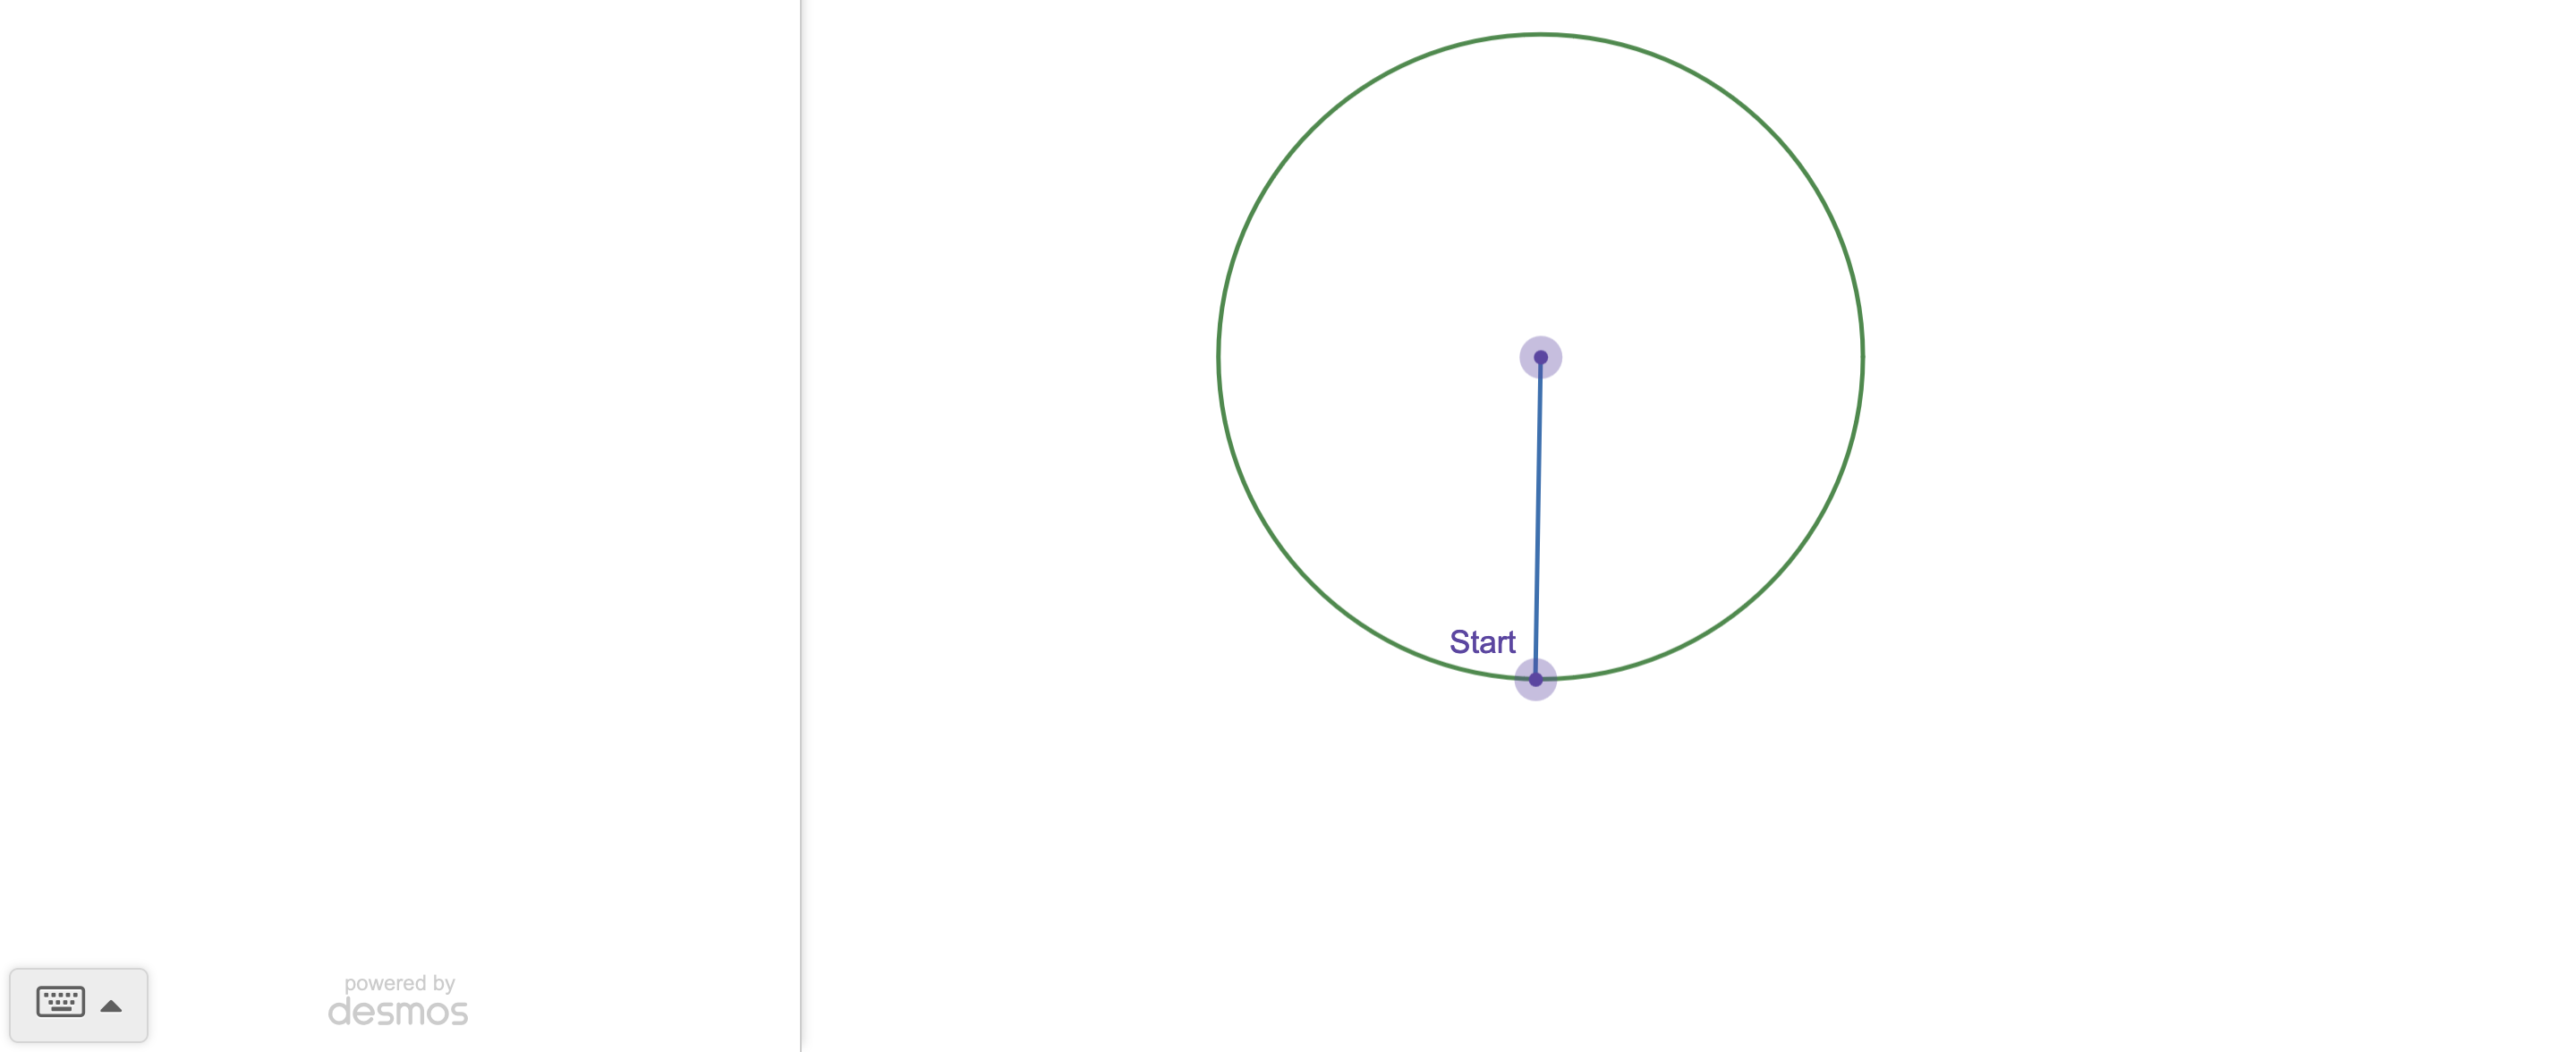
\includegraphics[width = 4in]{37}\newline Thus, after rotating $255^\circ$ more degrees, we have rotated $255+270=525$ degrees in total, which is coterminal with 
$525-360=165^\circ$, which is in Quadrant II, and thus has a reference angle of $180-165=15^\circ$. Hence the height $y$ of our position (relative to the circle) after the temporary stop is given by
\[ \sin 15^\circ=\frac{y}{75} \]
\[ y=75\sin 15^\circ \]
\[ y\approx 19.4 \]
meaning our height after the temporary stop is about $19.4+75+10=104.4$ feet. Suppose the radius $r$ was doubled (and that we still started 10 feet above the ground). Hence, for the wheel of radius $r$, the 
height above the ground after the temporary stop would be
\[ r\sin 15^\circ +r+10\approx 1.26r+10 \] and the height above the ground after the temporary stop for the radius of $2r$ would be
\[ 2r\sin 15^\circ +2r+10\approx 2.52r+10 \] which means that the height does not necessarily double. In fact, we can show that the height never doubles. For if it did, we would have
\[ 2.52r+10=2(1.26r+10) \]
\[ 2.52r+10=2.52r+20 \]
\[ 20=10 \] which is impossible.

\section*{38}
(a): 
We know that \[ \sin 117^\circ=\frac{y}{128} \]
\[ y=128\sin 117^\circ \]
\[ y\approx 114.05 \]
and \[ \cos 117^\circ=\frac{x}{128} \]
\[ x=128\cos 117^\circ \]
\[ x\approx -58.11 \] meaning the center of the oxygen atom in Quadrant II is about $(-58.11,114.05)$.


(b): Thus the distance between the two atoms is
\[ \sqrt{(-58.11-128)^2+(114.05-0)^2}\approx 218.28 \] picometers.

\section*{40}
We let $r_1$ be the radius of the earth, and $r$ be the radius of the circle of latitute $P$ which is half the distance around the equator, that is, half the circumference of the equator. From the diagram, if 
$\theta$ is the desired latitude, then we know that \[ \cos\theta =\frac{r}{r_1} \] \[ r=r_1\cos\theta \]
Also, because we know that the circumference of the circle with radius $r$ is half that of the circle with radius $r_1$,
\[ 2\pi r=\frac{2\pi r_1}{2}=\pi r_1 \]
\[ r=\frac{r_1}{2} \] 
Plugging this into the first equation, we recieve:
\[ \frac{r_1}{2}=r_1\cos\theta \]
\[ \dfrac{\frac{r_1}{2}}{r_1}=\cos\theta \]
\[ \cos\theta=\frac{1}{2} \] which means that $\theta=60^\circ$, that is, the latitude is $60^\circ$.

\end{document}
